\chapter{Theoretical Background}
\label{ch:theory}
\label{ch:chapter2}

This main of goal of this chapter is to present one theoretical model beyond the SM that introduces a vector leptoquark that could explain $B$-meson anomalies. However, before introducing such a model, some notions of quantum field theory (QFT) are outlined and applied in the context of the SM to serve as a relatively simple illustration of them, before using them in the construction of this new model.

This theoretical exposition begins with one of the most fundamental notions of modern particle physics: symmetry. Defining symmetry requires delving into the mathematical theory of groups. After a brief elucidation of the main aspects of group theory relevant for theoretical particle physics, special relativity is treated, aiming to understand the symmetry encoded in the Poincaré group. This serves as a stepping stone into the Dirac equation, which describes fermionic particles, and its interpretation as a quantum field. Then, the SM is introduced before dealing with physics beyond the SM, more concretely the 4321 model, in which vector leptoquarks arise as a gauge boson of the extended symmetry.

\section{Group theory}

As claimed before, symmetry is a key notion of particle physics, but one must make this concept precise in order to adequately incorporate it into the mathematical description of physical systems. Intuitively, symmetry is the absence of change under some ``transformation''. This intuitive picture of a symmetry imposes some behaviour on these ``transformations''. First and foremost since doing nothing always preserves the structure of any given object, we should include the identity transformation as a symmetry. Further, one would like to combine these ``transformations'' into antoher one that leaves the object unchanged. Finally, one must be able to go back on them; each symmetry should have an inverse. These properties are all encoded in mathematical objects known as groups.

\begin{newdef}
A group $G$ is a set endowed with a binary operation, $\cdot : G\times G \rightarrow G$, satisfying the following properties:
\begin{enumerate}
    \item for all $g,h,k\in G$, $g\cdot (h\cdot k) = (g\cdot h) \cdot k$,
    \item there is an element $e\in G$ such that $g\cdot e = e\cdot g = g$ for all $g\in G$,
    \item for all $g\in G$, there is an element $g^{-1} \in G$ such that $g \cdot g^{-1} = e$.
\end{enumerate}
\end{newdef}

Since groups encode symmetry, they can be naturally understood as acting on a given object, whose structure they preserve. In particular, the way groups operate on vector spaces preserving their structure is notably revealing about groups themselves. This motivates the notion of group representation.
\begin{newdef}
A representation of a group $G$ is a map, $T$, from $G$ onto a set of linear operators on a vector space, $V$, satisfying the following properties:
\begin{enumerate}
    \item $T(e) = I$, the identity operator on $V$,
    \item $T(g)T(h) = T(g\cdot h)$.
\end{enumerate}
\end{newdef}
In spite of being defined generally for all groups, representations are quite rigid. This definition requires the linear transformations in the image of the representation to be invertible, which also form a group denoted $GL(V)$. Additionally, these linear transformations should mirror the group structure in their behaviour under composition. 

Naturally, some representations are more useful than others. Consider for example the trivial representation which assigns the identity operator to each group element: $T(g) = I$, for all $g\in G$. This representation completely erases all information about the group structure. One class of interesting representations are those called \textit{irreducible}. A representation is said to be irreducible if there is no proper subspace $W\neq \{0\}$ of $V$ such that $T(g)w \in W$ for all $w\in W$ and $g\in G$. This entails that (if $V$ is finite-dimensional) the matrix representation of $T$ cannot be written in block-diagonal form.

Some symmetries are continuous, meaning they can be viewed as motions of some sort. To illustrate this point, consider the set symmetries of an equilateral triangle as opposed to those of a circle. The symmetries of the triangle can be seen as functions that take one corner to another (see fig. \ref{fig:triangle}). These symmetries and the group that describes them, $S_3$, are discrete. In contrast, the set of symmetries of a circle, which is just the set of 2D rotations, is continuous. Any 2D rotation may be regarded as continuous motion, unlike rotations of equilateral triangles, which are necessarily discrete.
\begin{figure}[t]
    \centering
    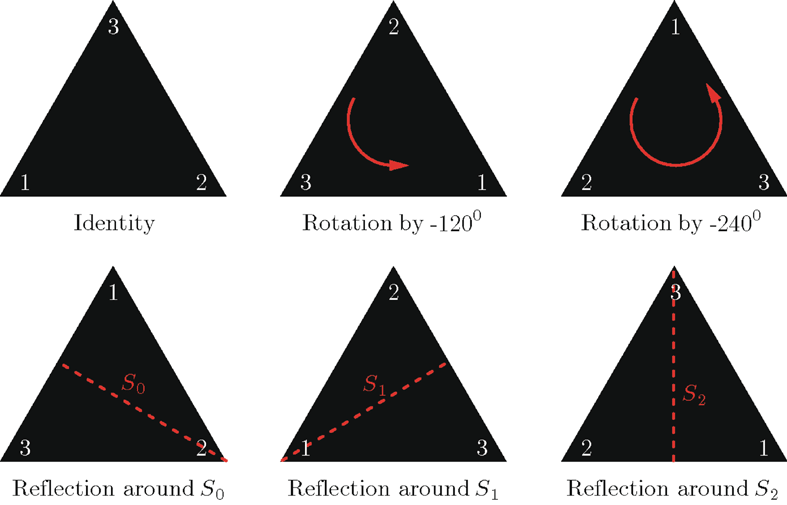
\includegraphics[width = 0.6\textwidth]{images/triangle_symmetries.png}
    \caption{Symmetries of an equilateral triangle (retrived from \cite{raviv_full_2010})}
    \label{fig:triangle}
\end{figure}

Groups describing continuous symmetries are also smooth manifolds. A smooth manifold $M$ is a topological space that locally resembles Euclidean space ($\mathbb{R}^n$) and admits differentiation of sorts. Smooth manifolds, in particular those describing continuous symmetries, can be parametrised by some (set of) continuous parameter(s). Groups endowed with a smooth manifold structure are called \textit{Lie groups}. Let $G$ be an $n$-dimensional Lie group, so elements close to the identity are parametrised by $n$ continuously varying numbers. Group elements can be written as $$g = g(\theta_1,\dotsc,\theta_n).$$ Due to its outstanding role within the group, the identity is usually identified by $\theta = 0$, $e = g(0)$. If a representation of $G$ is induced, these parameters also identify the linear operators, so $$T(g) = T(\theta_1,\dotsc,\theta_n).$$ Consider an element, $h$, arbitrarily close to the identity so its parameter, $\delta \theta = (\delta\theta_1,\dotsc,\delta\theta_n)$, is ``small''\footnote{Smallness is arbitrary. Thus, the description above is mathematically weak. For a rigorous treatment of Lie groups and algebras the reader may refer to \cite{tu_introduction_2011}.}. $h$ may be written as $$h = g(\delta \theta) = e+\delta\theta_i X_i,$$ where $X_i$ ($1\leq i \leq n$) are objects called generators (repeated indices imply summation over the repeated index, according to Einstein's summation convention). Other elements in the group, even those that cannot be considered close to the identity, can be obtained upon successive application of $h$, that is, $g = h^k$. In some representation, this implies $$T(g) = T(h^k) = [T(h)]^k = (I+\delta\theta_i X_i)^k.$$ If $g$'s parameter is $\theta$, take $\delta\theta = \lim_{k\to \infty} \theta/k$, so $$T(g) = \lim_{k\to \infty} \qty(I+\frac{\theta_i}{k} X_i)^k = e^{\theta_i X_i}.$$ This is how group elements are parametrised.

The continuous nature of the parameters can be leveraged to introduce a derivative, $D$. If $g = e^{\theta_i X_i}$, then its derivative is $$D[g(\theta)] = X_i e^{\theta_i X_i}.$$ Upon evaluating the derivative at the identity ($\theta = 0$), one obtains that $$ X_i = \pdv{g}{\theta_i}\eval_{\theta = 0}.$$ This serves as some sort of definition of the generators of a Lie group. This equation also shows that the generators are \textit{not} group elements, rather they belong to the tangent space of $G$.

A natural question arises when introducing Lie group generators: how are generators combined when two group elements are multiplied together? One may guess that given $g = e^X$ and $h = e^Y$, $g\cdot h = e^X\cdot e^Y = e^{X+Y}$. However, does not hold in general. Generators are combined according to the Baker-Campbell-Hausdorff formula \cite{schwichtenberg_physics_2017}: $$e^{X}\cdot e^{Y} = e^{X+Y+\comm{X}{Y}/2+\comm{X}{\comm{X}{Y}}/12-\comm{Y}{\comm{X}{Y}}/12+\dotsb},$$ where $\comm{\;}{\;}$ is a binary operation on the generators, called a Lie bracket. The Lie bracket satisfies the following properties:
\begin{enumerate}
    \item $\comm{aX+bY}{Z}=a\comm{X}{Y}+b\comm{Y}{Z}$,\newline $\comm{X}{aY+bZ}=a\comm{X}{Y}+b\comm{X}{Z}$;
    \item $\comm{Y}{X}=-\comm{X}{Y}$;
    \item $\comm{X}{\comm{Y}{Z}}+\comm{Z}{\comm{X}{Y}}+\comm{Y}{\comm{Z}{X}}=0$.
\end{enumerate}
The Lie bracket between generators is defined in a way that is consistent with multiplication in the group, thus the Lie bracket codifies the group structure. It can be shown that the set of generators of a Lie group is a vector space and the Lie bracket endows this vector space with an additional structure, that of an algebra. This algebra, called the Lie algebra, is unique to each Lie group and contains essentially the same information as the overall group but is much simpler to understand and work with. Before moving on to the application of this theory to physical reality, some examples of key groups in theoretical particle physics are reviewed.

\subsection{\texorpdfstring{$U(1)$}{U(1)}}
$U(1)$ is perhaps the simplest Lie group and is actually quite fundamental in particle physics. Simply stated, $U(1)$ is the group of unit-norm complex numbers: $$U(1) = \{e^{-i\theta}\,|\,\theta \in [0,2\pi) \}.$$ An irreducible representation of $U(1)$ is that of phase transformations: $$z \longmapsto e^{-i\theta}z.$$ The reader may have already encountered a $U(1)$-invariant theory: non-relativistic quantum mechanics. The phase of the quantum mechanical wave-function carries no physical meaning, so physical observations are invariant under phase shifts. A consequence of this symmetry is local probability conservation in the Born interpretation of quantum mechanics. As a matter of fact, any continuous symmetry implies a conservation law by Noether's theorem, which will be more carefully discussed in a later section.

The Lie algebra of this group is quite simple; there is only one linearly independent generator: $$ X = \dv{e^{-i\theta}}{\theta}\eval_{\theta = 0} = -i.$$
Since generators form a vector space, any scalar multiple of $X$ is also a generator. One may as well choose $iX = 1$ to be \textit{the} fundamental generator of the transformation. Since all generators are scalar multiples of each other, the Lie bracket is trivial: $$\comm{X}{Y} = 0\qc\text{for all $X,Y$ in the Lie algebra.}$$ The Baker-Campbell-Hausdorff formula implies that group elements combine according to $$e^{-i\theta}e^{-i\phi} = e^{-i(\theta+\phi)},$$ so evidently group elements commute.

Another irreducible representation of $U(1)$ is that of 2D rotations: $$e^{-i\theta} \longmapsto \mqty(\cos{\theta} & \sin{\theta} \\ -\sin{\theta} & \cos{\theta}).$$ Therefore, $U(1)$ is the group of symmetries of the circle.

\subsection{\texorpdfstring{$SU(2)$}{SU(2)}}\label{ss:SU2}
$SU(2)$ not only describes the fundamental symmetry of the weak interaction \cite{goldberg_standard_2017}, but also arises in special relativity \cite{schwichtenberg_physics_2017} and non-relativistic quantum mechanics. $SU(2)$ is the set of $2\times 2$ unit-determinant, unitary matrices. In symbols, $$SU(2) = \{ M \in M_{2\times 2}(\mathbb{C})\,|\, \det(M)=1,\ M^{\dagger} M = I\}.$$
There is a natural irreducible representation for $SU(2)$: left multiplication on $\mathbb{C}^2$. Let $$\phi = \mqty(\phi_1 \\ \phi_2) \qc \psi = \mqty( \psi_1 \\ \psi_2)$$ be vectors in $\mathbb{C}^2$. Under $SU(2)$ transformations, the inner product of $\phi$ and $\psi$ is invariant: $$ (M\phi)^{\dagger}(M\psi) = \phi^\dagger M^{\dagger} M \psi = \phi^{\dagger} \psi.$$ This is a consequence of unitarity.

Suppose $SU(2)$ elements are parmetrised by the matrix exponential $$ M = e^{\theta_i X_i},$$ where $X_i$ are linearly independent, complex $2\times 2$ matrices. 
Since $M$ is special, $$\det(M)=\det(e^{\theta_i X_i}) = 1,$$ but $\det(e^{A}) = e^{\Tr{A}}$, so $$\Tr(\theta_i X_i) = \theta_i\Tr(X_i) = 0.$$ This must hold for any value of $\theta_i$, so the immediate conclusion is that $\Tr(X_i)=0$. For unitarity to hold, $$ \qty(e^{\theta_i X_i})^{\dagger} e^{\theta_i X_i} = I,$$ but $(e^{tX})^\dagger = e^{tX^{\dagger}}$ according to \cite{hall_lie_2015}, so $$e^{\theta_i X_i^{\dagger}} = e^{-\theta_i X_i}.$$ This holds if and only if $X_i^{\dagger} = -X_i$. To dispose of the negative sign, the linearly independent set of generators is taken to be $J_i = iX_i$. One can immediately see that $$J_i^{\dagger} = (i X_i)^{\dagger} = -i X_i^{\dagger} = i X_i = J_i. $$ In quantum mechanics, one encounters a linearly independent set of matrices satisfying these properties, the Pauli matrices:
$$\sigma_1 = \mqty(\pmat{1})\qc \sigma_2 = \mqty(\pmat{2})\qc \sigma_3 = \mqty(\pmat{3}).$$ The fact that Pauli matrices are used to describe spin is no coincidence as shall be seen in section \ref{s:Dirac}.

The Lie bracket for the generators of $SU(2)$ (and actually any Lie group of matrices) is simply their commutator: $$\comm{A}{B} = AB-BA.$$ For the Pauli matrices, the commutation relations are $$\comm{\sigma_i}{\sigma_j} = 2i\epsilon_{ijk}\sigma_k.$$ To get rid of the factor of 2 in these commutation relations, basis elements for the Lie algebra of $SU(2)$, denoted $\mathfrak{su}(2)$, are taken to be $$J_i = \frac{1}{2}\sigma_i.$$ One thus obtains the commutation relations for quantum mechanical angular momentum. Again, this is no coincidence. It has to do with the fact that the Lie algebra of $SU(2)$ is isomorphic to that of $SO(3)$, the set of 3D rotations (plus handedness inversion). The proof of this statement is beyond the scope of this document (for further reference, see \cite{schwichtenberg_physics_2017}). This is enough group theory for the present document. From now on, this theory will be applied to concrete physical situations, starting with the theory of special relativity.

\section{Special Relativity}
The cornerstone of relativity is the idea that physical laws should be the same for all observers in uniform translational motion from one another. This idea motivated Einstein to develop the theory of special relativity \cite{griffiths_introduction_2018}. Einstein proposed two fundamental postulates:
\begin{enumerate}
    \item The laws of physics apply in all inertial reference frames.
    \item The speed of light in vacuum is the same for all inertial observers, regardless of the motion of the source.
\end{enumerate}

These postulates have profound geometrical consequences. The first is that space and time cannot be thought of as absolute. Instead, they are deeply intertwined with one another. Therefore, relativity introduces an amalgamation of the two, called space-time. Positions in this space-time are represented by quantities called 4-vectors: $$x^\mu = \mqty( ct \\ x \\ y \\ z),$$ where $c$ is the speed of light, $t$ is time and $x$, $y$, $z$ are three spatial coordinates (Greek indices run from 0 to 3). As the reader may recall from a course in special relativity, space and time coordinates transform from one inertial reference frame to a second reference frame moving with constant speed $v$ along the $x$ axis according to
\begin{align}
    t' &= \frac{1}{\sqrt{1-v^2/c^2}}\qty(t-\frac{v}{c^2}x), \label{eq:Lorentz_transfo_t}\\
    x' &= \frac{1}{\sqrt{1-v^2/c^2}}(x-vt), \label{eq:Lorentz_transfo_x}\\
    y' &= y, \label{eq:Lorentz_transfo_y}\\
    z' &= z. \label{eq:Lorentz_transfo_z}
\end{align}

This transformation can be cast in matrix form for the position 4-vector: $$x'^{\mu} = \mqty(\gamma & -\gamma\beta & 0 & 0 \\ -\gamma\beta & \gamma & 0 & 0 \\ 0 & 0 & 1 &0 \\ 0 & 0 & 0 & 1)x^\mu, $$ where $\gamma = (1-v^2/c^2)^{-1/2}$ and $\beta = v/c$. This transformation is an example of a \textit{Lorentz transformation}. Lorentz transformation matrices are denoted by ${\Lambda^{\mu}}_{\nu}$.

4-vectors are defined beyond position as any 4-component quantity that transforms like space-time position does. 4-vectors come with an inner product that is invariant under the transformations of \eqref{eq:Lorentz_transfo_t} - \eqref{eq:Lorentz_transfo_z}. The inner product of two 4-vectors $a^\mu$ and $b^\mu$ is $$ a^0b^0-a^1b^1-a^2b^2-a^3b^3.$$ To simplify notation, one introduces the Minkowski metric, $$ g_{\mu\nu} = \mqty(\dmat[0]{1,-1,-1,-1}),$$ and uses Einstein's summation convention, so the inner product can be written as $$g_{\mu\nu} a^\mu b^\nu.$$ Notation is even simpler using covariant vectors, denoted $a_\mu$, and defined by $a_\mu = g_{\mu\nu}a^\nu$. Thus, the inner product is denoted simply by 
\begin{equation}
    a^{\mu}b_{\mu}.
\end{equation}

The 4-vector inner product is another invariant quantity when transforming reference frames. Actually, this inner product is invariant under a more general class of transformations, called Lorentz transformations\footnote{In fact, the inner product is also invariant under space-time translations. The group containing the Lorentz group and space-translations is known as the Poincaré group.}. Lorentz transformations not only include transformations between inertial reference frames (also known as Lorentz boosts) but also under spatial rotations, parity inversion ($x^i \mapsto -x^i$, Latin indices run from 1 to 3), and time reversal ($x^0\mapsto -x^0$). Lorentz transformations form a group, known as the Lorentz group, denoted $O(1,3)$. The fact that the inner product is Lorentz invariant implies something about the metric, namely, that \begin{equation}\label{eq:metric_Lorentz_trans}
    {\Lambda^\mu}_{\rho} g^{\rho\sigma} {\Lambda^{\nu}}_{\sigma} = g^{\mu\nu}.
\end{equation}

To characterise the Lorentz Lie algebra, consider an infinitesimal Lorentz transformation, $${\Lambda^{\mu}}_{\nu} = {\delta^{\mu}}_\nu+{\omega^\mu}_\nu.$$ According to \eqref{eq:metric_Lorentz_trans},
\begin{align*}
    {\Lambda^{\mu}}_{\rho}{\Lambda^{\nu}}_{\sigma} g^{\rho\sigma} &= \qty({\delta^{\mu}}_\rho+{\omega^\mu}_\rho)\qty({\delta^{\nu}}_\sigma+{\omega^\nu}_\sigma) g^{\rho\sigma}\\
    &= \delta^{\mu\nu}+\omega^{\nu\mu}+\omega^{\mu\nu}+\mathcal{O}(\omega^2) = g^{\mu\nu}.
\end{align*}
Since the metric tensor is 0 order with respect to $\omega$ and $\omega$ is infinitesimal, this condition reduces to $$ \omega^{\mu\nu} = -\omega^{\nu\mu}.$$ Since Lorentz transformations act on 4-vectors, suppose $\omega$ is a $4\times 4$ matrix. An anti-symmetric matrix of said size has $4\times 3/2 = 6$ free parameters, corresponding to the 6 parameters of Lorentz transformations: 3 for rotations and 3 for boosts. The Lie algebra of $O(1,3)$ has a basis consisting of 6 $4\times 4$ anti-symmetric matrices. These matrices are labeled by a pair of anti-symmetric indices, $\rho,\sigma$, running from 0 to 3, $M^{\rho\sigma}$. The basis elements can be written as $${(M^{\rho\sigma})^{\mu}}_\nu = g^{\rho\mu}{\delta^{\sigma}}_\nu-g^{\sigma\mu}{\delta^{\rho}}_{\nu}.$$ These are the generators of the Lorentz transformations. Hence, Lorentz transformations\footnote{A caveat to this statement: not \textit{every} Lorentz transformation can be written this way. Lorentz transformations that invert time or handedness cannot be parametrised this way. This has to do with the fact that the Lorentz group is not simply connected, and thus one requires discrete transformations to obtain such transformations. Lorentz transformations that follow this parametrisation belong to the proper orthochronous Lorentz group.} can be written as $$\Lambda = \exp(\frac{1}{2}\Omega_{\rho\sigma}M^{\rho\sigma}), $$ where $\Omega_{\rho\sigma}$ are six parameters for the Lorentz transformation.

It can be shown that the generators obey the commutation relations 
\begin{equation}\label{eq:Lorentz-algebra}
    \comm{M^{\rho\sigma}}{M^{\lambda \kappa}} = g^{\sigma\lambda}M^{\rho\kappa}-g^{\rho\lambda}M^{\sigma\kappa}+g^{\rho\kappa}M^{\sigma\lambda}-g^{\sigma\kappa}M^{\rho\lambda}.
\end{equation}
This commutation relation defines the Lie algebra of the Lorentz group.

The Lorentz group has several representations. One of the simplest is the Lorentz transformation of scalar fields defined on space-time. Scalar fields are simply functions that assign to each point in space-time a number (it might be a complex number). Let $\phi(x)$ be such a field. The Lorentz group acts on the set of space-time positions by $x^{\mu} = {\Lambda^{\mu}}_{\nu} x^{\nu}$, so $x\mapsto \Lambda x$. For the field, $\phi(x) \mapsto \phi(\Lambda^{-1} x)$. The inverse means that the new field is written in terms of the old field by simply evaluating it in the point that maps to $x'$. This point is best illustrated when considering a rotation. Suppose $\phi(x)$ has its maximum value at $\Vec{x} = (1,0,0)$. After a \ang{90} rotation in the $xy$-plane, the maximum is now achieved at $\Vec{x}=(0,1,0)$. In symbols, $$\phi'(0,1,0)= \phi(R^{-1}(0,1,0)) = \phi(1,0,0).$$ An interesting point to be made is that if the equations of motion of the field include terms of the form $\dcov \phi \dcon \phi$, where $\dcov = (c^{-1}\pdv*{t},\grad)$, they are also Lorentz invariant. Since Lorentz transformations satisfy \eqref{eq:metric_Lorentz_trans}, $\dcov \phi \dcon \phi$ transforms according to
\begin{align*}
    \dcov \phi(x) \dcov[\nu] \phi(x) g^{\mu\nu} \longmapsto & {(\Lambda^{-1})^{\rho}}_{\mu} \dcov[\rho] \phi(\Lambda^{-1}x) {(\Lambda^{-1})^{\sigma}}_{\mu} \dcov[\sigma] \phi(\Lambda^{-1}x) g^{\mu\nu}\\
    & \dcov[\rho] \phi(\Lambda^{-1}x) \dcov[\sigma] \phi(\Lambda^{-1}x) g^{\rho\sigma}.
\end{align*}
Fields of this form describe spin 0 particles \cite{peskin_introduction_1995}. However, in the present work no spin 0 particles are directly involved, so these types of fields will not be further discussed.

The set of Lorentz boosts may be regarded as a set of ``hyperbolic rotations'', so $O(1,3)$ is a combination of two ``rotation groups''. As stated at the end of subsection \ref{ss:SU2}, the Lie algebra of the group of 3D rotations is isomorphic to $\mathfrak{su}(2)$, so, in a way, the Lorentz group corresponds to two copies of $SU(2)$. Some irreducible representations of these two copies of $SU(2)$ act on a set of two-component objects called spinors. One copy of $SU(2)$ acts on left-chiral spinors and the other on right-chiral spinors. Left- and right-chiral spinors can be merged together into 4-component objects called bispinors \cite{schwichtenberg_physics_2017}. Bispinors and chirality will be treated with more detail in the following section, after introducing the Dirac equation.

More interesting representations can be defined, giving way to particles with nonzero spin. A somewhat more complicated example is the representation on vector fields, like the electromagnetic 4-vector potential, $A^\mu$:
\begin{equation}\label{eq:vector_Lorentz_trans}
    A^\mu(x) \longmapsto {\Lambda^{\mu}}_{\nu} A^{\nu} (\Lambda^{-1} x).
\end{equation}
Fields that transform like this describe spin 1 particles, such as the photon and other vector bosons \cite{peskin_introduction_1995}. 

\section{The Dirac Equation}\label{s:Dirac}

In what follows, the focus is shifted towards producing equations of motion for bispinors, $\psi$. A first approach is to assume $\psi$ corresponds to a multi-component wave function, so it evolves according to Schrödinger's equation,
\begin{equation}\label{eq:Schroedinger}
    H \psi = i\hbar \pdv{\psi}{t},
\end{equation}
where $H$ is the Hamiltonian. A first approach in writing a relativistic Hamiltonian is Einstein's energy relation, $$ H = \sqrt{c^2p^2+m^2c^4}.$$ However, in a quantum mechanical treatment, momentum becomes an operator and the square root of an operator is ill-defined. To solve this issue, Dirac suggested a Hamiltonian of the form $$H = c\alpha_ip_i+\beta mc^2,$$ where $\alpha_i$ and $\beta$ are matrices determined by $H^2 = c^2p^2 + m^2c^4$: 
\begin{align*}
    c^2(p_x^2+p_y^2+p_z^2) + m^2c^4 =& \qty[c^2(\alpha_x^2 p_x^2+\alpha_y^2 p_y^2+ \alpha_z^2 p_z^2)+\beta^2 m^2c^4]\\
    &\quad + \qty[c^2p_xp_y(\alpha_x\alpha_y+\alpha_y\alpha_x)+ c^2p_xp_z(\alpha_x\alpha_z+\alpha_z\alpha_x)+c^2p_yp_z(\alpha_y\alpha_z+\alpha_z\alpha_y)]\\
    &\quad + \qty[mc^3p_x(\alpha_x\beta+\beta\alpha_x)+mc^3p_y(\alpha_y\beta+\beta\alpha_y) + mc^3p_z(\alpha_z\beta+\beta\alpha_z)].
\end{align*}
This equation implies that
\begin{align*}
    \alpha_i^2 &= \beta^2 = 1 \quad (i=x,y,z),\\
    \alpha_i\alpha_j + \alpha_j \alpha_i &= \pb{\alpha_i}{\alpha_j} = 0 \quad (i\neq j),\\
    \alpha_i\beta +\beta \alpha_i &= \pb{\alpha_i}{\beta} = 0.
\end{align*}
The matrices $\alpha_i$ and $\beta_i$ should be Hermitian, traceless, and have eigenvalues $\pm 1$. One can obtain four (or more) linearly independent matrices satisfying these properties if their size is at least $4\times 4$ \cite{shankar_principles_1994}.

These conditions are satisfied if $\alpha_i = \gamma^0 \gamma^{i}$ and $\beta = \gamma^0$, where $\gamma^\mu$ are $4\times 4$ complex matrices satisfying the Clifford algebra:
\begin{align}
    \pb{\gamma^\mu}{\gamma^\nu} &= 2g^{\mu\nu} I, \label{eq:Clifford_alg1}\\
    (\gamma^0)^2 = I, & \qquad (\gamma^i)^2 = -I. \label{eq:Clifford_alg2}
\end{align}
Using the $\gamma$-matrices, the Hamiltonian becomes $$H = \gamma^0(c\gamma^i p_i+mc^2).$$ Substituting into \eqref{eq:Schroedinger} and letting $p_i \to -i\hbar \pdv*{x_i}$, $$\gamma^0\qty[ c\gamma^i \qty(-i\hbar\pdv{x_i})+mc^2]\psi = i\hbar \pdv{\psi}{t}.$$ Multiply both sides by $\gamma^0$ and divide by $c$ so, 
\begin{gather*}
    i\hbar\qty(\gamma^0 \frac{1}{c}\pdv{\psi}{t}+\gamma^{1}\pdv{x}+\gamma^{2}\pdv{y}+\gamma^{3}\pdv{z})\psi-mc \psi = 0
\end{gather*}
Introducing $\dcov$ and Einstein's summation convention, this equation becomes
\begin{equation}\label{eq:Dirac}
    \qty(i\hbar \gamma^\mu \dcov - mc)\psi = 0.
\end{equation}
This is the Dirac equation. In what remains of this document, natural units are used, so $\hbar = c = 1$ and Dirac's equation takes the form
\begin{equation}\label{eq:Dirac_nu}
    (i\slashed{\partial}-m)\psi = 0,
\end{equation}
where $\slashed{\partial} \equiv \gamma^\mu \dcov$. This equation determines the evolution of the spinors.

In the last two sections, two seemingly unrelated algebras have been introduced: the Clifford algebra and the Lorentz algebra. However, upon closer inspection there is a connection between the two. Consider the commutator of two $\gamma$-matrices, $$S^{\mu\nu} = \frac{1}{4}\comm{\gamma^\mu}{\gamma^\nu}.$$ By repeated application of \eqref{eq:Clifford_alg1}, one may show that these matrices satisfy the commutation relations \eqref{eq:Lorentz-algebra}. Therefore, the matrices $S^{\mu\nu}$ form a representation of the Lorentz algebra complexification. Denote this representation by $S[\Lambda]$. 

It remains to be seen that this representation actually behaves like two copies of $SU(2)$ as stated in the previous section. With this goal in mind, a concrete representation of the $\gamma$-matrices must be introduced. Such a representation, in $2\times 2$ block form, could be
$$\gamma^0 = \mqty(\admat[0]{I,I}), \quad \gamma^{i} = \mqty(\admat[0]{\sigma_i,-\sigma_i}).$$ This representation is known as chiral or Weyl representation. Now, consider bispinor behaviour under concrete transformations. The simplest case is that of rotations. There are three rotation generators, which correspond to $S^{\mu\nu}$ matrices with both spatial indexes:
\begin{align*}
    S^{ij} &= \frac{1}{4}\comm{\gamma^{i}}{\gamma^{j}} = \frac{1}{4}\qty[\mqty(\admat[0]{\sigma_{i},-\sigma_i})\mqty(\admat[0]{\sigma_{j},-\sigma_j})-\mqty(\admat[0]{\sigma_{j},-\sigma_j})\mqty(\admat[0]{\sigma_{i},-\sigma_i})]\\
    &= \frac{1}{4}\qty[\mqty(\dmat[0]{-\sigma_i\sigma_j, -\sigma_i\sigma_j})-\mqty(\dmat[0]{-\sigma_j\sigma_i, -\sigma_j\sigma_i})] \\
    &= -\frac{i}{2}\epsilon^{ijk}\mqty(\dmat[0]{\sigma_k,\sigma_k}).
\end{align*}
If $\theta^i$ are three angles to parametrise 3D rotations, such as the Euler angles, let $\Omega_{ij} = -\epsilon_{ijk}\theta^{k}$, so $$S[\Lambda] = \exp(\frac{1}{2}\Omega_{ij}S^{ij}) = \mqty(\dmat[0]{e^{i\theta^i \sigma_i/2},e^{i\theta^i \sigma_i/2}}).$$ The upper two components of the spinor and the lower two components transform according to the $SU(2)$ representation.

On the other hand, boosts are generated by $S^{\mu\nu}$ matrices with one index equal to zero and the other a spatial index:
\begin{align*}
    S^{0i} &= \frac{1}{4}\comm{\gamma^{0}}{\gamma^{i}} = \frac{1}{4}\qty(\gamma^0\gamma^i-\gamma^i\gamma^0) = \frac{1}{2}\gamma^0\gamma^i\\
    &=\frac{1}{2}\mqty(\admat[0]{I,I})\mqty(\admat[0]{\sigma_{i},-\sigma_i}) = \frac{1}{2}\mqty(\dmat[0]{-\sigma_i,\sigma_i}).
\end{align*}
Let $\beta_i$ be three parameters for the boosts and define $\Omega_{0i} = -\beta_i$, so the bispinor boost matrix is $$ S[\Lambda] = \exp(\frac{1}{2}\Omega_{0i}S^{0i}) = \mqty(\dmat[0]{e^{\beta_i\sigma^i/2},e^{-\beta_i\sigma^i/2}}).$$
It is finally evident the way the Lorentz group separates into two copies of $SU(2)$. It is customary to separate spinors by the part that is affected by each block, $$ \psi = \mqty( \psi_L \\ \psi_R).$$ The two component objects $\psi_L$ and $\psi_R$ are called left- and right-handed Weyl spinors. The 4-component bispinor is called a Dirac spinor \cite{peskin_introduction_1995}. The meaning right- and left-handedness should be clarified after considering explicit solutions of the Dirac equation.


\subsection{Solutions of the Dirac Equation}
In order to understand the physics of the Dirac equation, some solutions of the Dirac equation are produced. Consider a particle at rest, so the Dirac equation reads $$i\gamma^0\pdv{\psi}{t}-m\psi = 0.$$ Using the chiral representation for $\gamma^0$ and the Weyl spinors, this equation becomes
\begin{align*}
    i\pdv{\psi_L}{t}-m\psi_R &= 0, \\
    i\pdv{\psi_R}{t}-m\psi_L &= 0.
\end{align*}
This system of equations yields four linearly independent solutions: $$u_{+}(x)= N\mqty(1 \\ 0 \\ 1 \\ 0)e^{-imt}\qc u_{-}(x)= N\mqty(0 \\ 1 \\ 0 \\ 1)e^{-imt}\qc v_{-}(x)= N\mqty(1 \\ 0 \\ -1 \\ 0)e^{imt}\qc v_{+}(x)= N\mqty(0 \\ 1 \\ 0 \\ -1)e^{imt}. $$ Recalling that $H\psi = i\pdv*{\psi}{t}$, one gets that $H u_{s} = mu_{s}$ and $H v_{s} = -mv_{s}$, where $s$ serves as a label, whose physical significance will be clarified after noting the following: the Dirac equation admits negative energy solutions. This is clearly a problem if the Dirac spinor is to be interpreted as a single-particle wave function.

Moreover, focusing on the positive-energy solutions, the upper component and lower components of $u_{+}$ behave under 3D rotations just like a spin up particle, while the same components of $u_{-}$ behave like a spin down particle. This is the physical significance of the $s$ label.

Explicit solutions for the general case, in which the particle is moving with 4-momentum $(E,\vec{p})$, can be obtained by boosting these rest-frame solutions. This calculation is omitted here but the reader may refer to \cite{peskin_introduction_1995} to see how it is done. Instead the problem of negative energy solutions is addressed by giving the Dirac spinor a quantum field interpretation.

\section{Quantising the Dirac Field}

The previous section showed that the Dirac equation, as a single-particle theory, admits negative energy eigenvalues. This entails that perturbations may induce transitions into lower and lower energy states. This issue is solved by introducing quantum fields. Moreover, quantum fields allow for the creation and annihilation of particles, a fact that can be leveraged to describe particle physics. This section is devoted to examining key aspects of classical field theory that will be needed for a subsequent discussion of quantum fields. Afterwards, the Dirac field is quantised, following the approach of \cite{lahiri_first_2005}.

\subsection{Classical Field Theory}\label{ss:classical_ft}
A field is a quantity defined at every point of space-time $(t,\Vec{x})$. While classical particle mechanics is interested in describing a system via a set of generalized coordinates $q_a(t)$, indexed by $a$, field theory concerns itself with the dynamics of fields, $$\phi_a(\Vec{x},t),$$ where both $\Vec{x}$ and $a$ are labels. The label $a$ has the same role as in classical particle mechanics. Different values of $a$ can stand for completely independent fields or for different members of a set of fields related by some internal constraint or symmetry \cite{lahiri_first_2005}.

\subsubsection*{Euler-Lagrange equations}
In analogy with classical mechanics, the dynamics of a field are governed by a Lagrangian function, that is a function of $\phi(\Vec{x},t)$, $\Dot{\phi}(\Vec{x},t)$ and $\grad{\phi}(\Vec{x},t)$. The Lagrangian is of the form $$L(t)=\int \dd{^3x}\mathcal{L}(\phi_a,\partial_\mu\phi_a),$$ where $\mathcal{L}$ is the Lagrangian \textit{density}. The action is then defined as the integral of the Lagrangian function over time. Written explicitly that is \cite{lahiri_first_2005} $$S=\int_{t_1}^{t_2}\dd{t}\int\dd{^3x}\mathcal{L}(\phi_a,\partial_\mu \phi_a)=\int\dd{^4x}\mathcal{L}.$$

As is the case for classical Lagrangian mechanics, the equations of motion are determined by the principle of least action: the fields evolve such that the action has a stationary value. So if the fields are varied by an arbitrary function $\delta\phi_a(x)$ that vanishes at the space-time boundary (i.e. $\delta\phi_a(\Vec{x},t_1)=\delta\phi_a(\Vec{x},t_2)=0$), the corresponding variation in the action $\delta S$ is zero.
\begin{align*}
    \delta S &= \int\dd{^4x}\qty[\pdv{\mathcal{L}}{\phi_a}\delta\phi_a+\pdv{\mathcal{L}}{(\partial_\mu \phi_a)}\delta(\partial_\mu\phi_a)]\\
    &=\int \dd{^4x}\qty[\pdv{\mathcal{L}}{\phi_a}\delta\phi_a-\partial_\mu\qty(\pdv{\mathcal{L}}{(\partial_\mu \phi_a)})]\delta\phi_a+\int\dd{^4x}\partial_\mu\qty(\pdv{\mathcal{L}}{(\partial_\mu\phi_a)}\delta\phi_a)
\end{align*}
By Gauss' theorem, the last term becomes a surface integral on the boundary, but the variation $\delta\phi_a$ vanishes there, so the integral is equal to zero. For the other term to be equal to zero for \textit{any} $\delta\phi_a$, the term in between brackets must be zero. Thus the Euler-Lagrange equation is obtained \cite{peskin_introduction_1995}:
\begin{equation}
    \partial_\mu\qty(\pdv{\mathcal{L}}{(\partial_\mu \phi_a)})-\pdv{\mathcal{L}}{\phi_a}=0.
\end{equation}
\subsubsection*{Noether's Theorem}

The guiding principle of this present document is that of symmetry. In this exposition of field theory, symmetry seems to have vanished into the realm of abstract group theory. It is time to bring it back to the forefront of the discussion. The role of symmetry in field theory is summarised in Noether's theorem. It relates continuous symmetries of the Lagrangian to conservation laws.

Before stating Noether's theorem, we must define a continuous symmetry of the Lagrangian. A continuous symmetry is a variation of the fields $\phi_a\rightarrow \phi_a'= \phi_a+\delta\phi_a$ such that the Lagrangian varies by a total derivative, $$\mathcal{L}(\phi_a',\dcov \phi_a')=\mathcal{L}(\phi_a,\dcov\phi_a)+\dcov F^\mu,$$ and the action is left invariant, $$S=\int\dd{^4x}\mathcal{L}=\int\dd{^4x}\qty(\mathcal{L}+\dcov F^\mu).$$
The stage is set to state and prove Noether's theorem in field version \cite{peskin_introduction_1995}.
\begin{thm}
Every continuous symmetry of a Lagrangian implies the existence of a conserved current $j^{\mu}$.
\end{thm}
\begin{proof}
Consider the variation on the Lagrangian under an arbitrary variation of the fields $\delta\phi_a$:
\begin{align*}
    \var{\mathcal{L}}&=\pdv{\mathcal{L}}{\phi_a}\var{\phi_a}+\pdv{\mathcal{L}}{(\dcov\phi_a)}\dcov(\var{\phi_a})\\
    &=\qty[\pdv{\lag}{\phi_a}-\dcov\pdv{\lag}{(\dcov\phi_a)}]\var{\phi_a}+\dcov\qty(\pdv{\lag}{(\dcov\phi_a)}\var{\phi_a}).
\end{align*}
When the equations of motion are satisfied, the term in square brackets is zero. So the variation of the Lagrangian is just $$ \var{\lag}=\dcov\qty(\pdv{\lag}{(\dcov\phi_a)}\var{\phi_a}).$$ But by definition, for a symmetry $\var{\lag}=\dcov F^{\mu}$. Letting $\var{\phi_a}=X_a(\phi)$ and equating this with the last expression, gives the result $$\dcov j^\mu = 0\qq{with} j^{\mu}=\pdv{\lag}{(\dcov\phi_a)}X_a(\phi)-F^\mu(\phi).$$
\end{proof}
Conserved currents given Noether's theorem are known as Noether currents. Notice that the local conservation of a Noether current, stated mathematically as $\dcov j^\mu = 0$, implies the global conservation of an associated charge, $$Q = \int d^3 x j^0,$$ by Gauss' theorem.

To see Noether's theorem in action consider an infinitesimal space-time translation: $$x^{\mu} \mapsto x^{\mu}-\epsilon^{\nu}.$$ The field transforms according to $$\phi_a (x) \longmapsto \phi_a(x) + \epsilon^{\nu} \dcov[\nu] \phi_a(x).$$ On the other hand, the Lagrangian itself transforms as $$\lag(x) \longmapsto \lag(x) + \epsilon^{\nu} \dcov[\nu] \lag(x).$$ Since the change in the Lagrangian is a total derivative, by Noether's theorem four conserved currents are obtained, one for each translation parameter $\epsilon^\nu$: $$(j^\mu)_\nu = \pdv{\lag}{(\dcov\phi_a)}\dcov[\nu]\phi_a-{\delta^\mu}_{\nu}\lag.$$ This equation defines the energy-momentum tensor ${T^\mu}_{\nu}$. The conserved charges will be worked out after introducing the Hamiltonian formalism for fields.

% A final remark on Noether's theorem: continuous symmetries are associated with Lie groups, so what is the relationship between Lie groups and Noether currents? Suppose an element of a Lie group acts on the fields. For the variation of the field to be considered small, the group element must be infinitesimal, thus the fields change by $$\phi_a \longmapsto \phi_a + \theta_i X_i \phi_a.$$ Now, for a given configuration of the fields, the Lagrangian transforms according to $$\lag(x) \longmapsto \lag(x) + \sum_{i}\dcov \lag(x) \pdv{x^\mu}{\theta_i} \theta_i,$$ by the chain rule. Assuming $\pdv*{x^\mu}{\theta_i}$ is divergenceless ($\dcov (\pdv*{x^\mu}{\theta_i})=0$), the variation of the Lagrangian is simply $$\var{\lag} = \theta_i \dcov\qty(\pdv{x^\mu}{\theta_i}\lag).$$ Thus, the Noether currents are simply $$(j^\mu)_i = \pdv{\lag}{(\dcov \phi_a)}X_i\phi_a - \pdv{x^\mu}{\theta_i}\lag.$$ This will become extremely relevant when analysing the internal symmetries of the SM.

\subsubsection*{Hamiltonian Formalism}
In order to formulate a quantum theory out of its classical counterpart, the Hamiltonian formalism is often more useful \cite{peskin_introduction_1995}. The basis of such formalism is naturally the momentum. The momentum $\pi^a(x)$ conjugate to $\phi_a(x)$ is defined as $$\pi^a(x)=\pdv{\lag}{\Dot{\phi}_a}.$$ The \textit{Hamiltonian density} is given by $$\mathcal{H}=\pi^a(x)\Dot{\phi}_a(x)-\mathcal{L},$$ where, as in classical mechanics, $\Dot{\phi}_a(x)$ is eliminated everywhere in favour of $\pi^a(x)$ everywhere in $\mathcal{H}$. $\mathcal{H}$ carries physical meaning as the energy density of the fields. To obtain the total energy or the Hamiltonian, one must integrate the Hamiltonian density over all of space: $$ H=\int\dd{^3x}\mathcal{H}.$$

Returning to the energy-momentum tensor, notice that
$$T^{00} = \pdv{\lag}{(\partial_t \phi_a)}\partial_t \phi_a- \lag = \pi^a \Dot{\phi}_a(x)-\lag = \mathcal{H},$$ so the conserved charge is $$ \int T^{00} d^3 x = \int \dd{^3 x} \mathcal{H} = H.$$ The conserved charge associated with time translations is the Hamiltonian. The conserved charges associated with spatial translations are $$ P^i = \int T^{0i} d^3 x = \int -\pdv{\lag}{(\partial_t \phi_a)}\partial_{i} \phi_a \,d^3x = -\int \pi^a \partial_{i} \phi_a \,d^3x,$$ which is naturally interpreted to be momentum carried by the fields.

\subsection{Quantum fields}

The procedure for quantising fields is similar to that of quantising a classical theory. Quantum mechanics is obtained from its classical counterpart by promoting generalised coordinates and momenta to operators. A prototype of this procedure is the quantisation of the harmonic oscillator. The Hamiltonian in the classical case is $$ H = \frac{p^2}{2m} + \frac{1}{2}m\omega^2 x^2,$$ where $p$ is the momentum and $x$ the position. Upon quantisation, $x$ and $p$ become operators, denoted by upper case letters, on the Hilbert space of quantum states, so $$ H = \frac{1}{2m}P^2+\frac{1}{2}m\omega^2 X^2.$$ Commutation relations between the operators are defined according to the Poisson bracket of the classical theory. For position and momentum, this means $\comm{X}{P} = i$ (recall $\hbar = c = 1$).

One can define a pair of operators
\begin{align}
    a &= \qty(\frac{m\omega}{2})^{1/2}X+i\qty(\frac{1}{2m\omega})^{1/2} P, \\
    a^{\dagger} &= \qty(\frac{m\omega}{2})^{1/2}X-i\qty(\frac{1}{2m\omega})^{1/2} P.
\end{align}
Using the commutation relation for $X$ and $P$, it can be shown that $\comm{a}{a^{\dagger}} = I$. These operators are related to the Hamiltonian by
\begin{align*}
    a^{\dagger} a &= \frac{m\omega}{2}X^2+\frac{1}{2m\omega}P^2+\frac{i}{2}\comm{X}{P}\\
    &= \frac{H}{\omega}-\frac{1}{2},
\end{align*}
so
\begin{equation}
    H = \omega(a^{\dagger}a+1/2).
\end{equation}
It can be easily shown that $$\comm{H}{a^{\dagger}} = \omega a^{\dagger}\qand \comm{H}{a} = -\omega a.$$ Let $\ket{\varepsilon}$ be an eigenstate of $H$, so $H\ket{\varepsilon} = \varepsilon \ket{\varepsilon}$. To understand the importance of $a$ and $a^{\dagger}$, consider
\begin{align*}
    Ha\ket{\varepsilon} &= (aH-\comm{a}{H})\ket{\varepsilon}\\
    &= (aH-\omega a)\ket{\varepsilon}\\
    &= (\varepsilon-\omega) a\ket{n}.
\end{align*}
It is then clear that $$ a\ket{\varepsilon} = C\ket{\varepsilon-\omega}.$$ It can be similarly shown that $$ a^{\dagger}\ket{\varepsilon} = D\ket{\varepsilon+\omega}.$$ Therefore, $a^{\dagger}$ and $a$ are known as raising and lowering operators. This implies that if one eigenstate of the oscillator is known, others can be found by simple application of $a^{\dagger}$ and $a$.

Since the energy of the harmonic oscillator is bounded below, $a$ cannot be applied multiple times to find eigenstates with increasingly lower energy. Instead, there is a ground state, $\ket{\varepsilon_0}$ such that $a\ket{\varepsilon_0} = 0$. Operating with $a^{\dagger}$, $$a^{\dagger} a\ket{\varepsilon_0} = \qty(\frac{H}{\omega}-\frac{1}{2}) \ket{\varepsilon_0} =0 ,$$ so $$H\ket{\varepsilon_0} = \frac{1}{2}\omega\ket{\varepsilon_0}.$$ $\ket{\varepsilon_0} \equiv \ket{0}$ is known as the ground state. All other eigenstates can be found by repeated application of $a^{\dagger}$: $$\ket{n} = (a^{\dagger})^n \ket{0}, \quad \text{with}\ H\ket{n} = (n+1/2)\omega\ket{n}.$$


In field theory, the fields themselves are promoted to operators. To that end, the same trick as with the quantum oscillator is applied. However, fields have several oscillation modes with different frequencies, so each one must have its own creation and annihilation operators. As a consequence, the fields must be written as a Fourier decomposition of the plane-wave solutions for the field with creation and annihilation operators as coefficients. This is illustrated for the Dirac field.

\subsubsection*{Dirac Equation in Quantum Field Theory}
Plane-wave solutions for the Dirac equation come in four types, $u_{\pm}$ and $v_{\pm}$. Fixed-momentum solutions of the Dirac equation are linear combinations of these four linearly independent solutions for the Dirac equation:
$$\psi_p(x) = \sum_{s} b_{s} u_{s}(p)e^{-ip\cdot x}+ c_{s} v_{s}(p) e^{ip\cdot x}.$$ Arbitrary momentum solutions are obtained by integrating over all possible momenta:
$$\psi(x) = \int \frac{d^4 p}{(2\pi)^4} \sum_{s} \qty[ b_{s}(p) u_{s}(p)e^{-ip\cdot x}+ c_{s}(p) v_{s}(p) e^{ip\cdot x}].$$ However, the 4-momentum components are not all free, they must satisfy the energy-momentum relation $E^2-p^2 = m^2$. To guarantee this holds, a $\delta$-function is inserted in the integral. 
\begin{align*}
    \psi (x) &= \int \frac{d^4 p}{(2\pi)^3} \delta((p^0)^2-p^2)\sum_{s} \qty[ b_{s} u_{s}(p)e^{-ip\cdot x}+ c_{s} v_{s}(p) e^{ip\cdot x}] \\
    &= \int \frac{d^4 p}{(2\pi)^3\sqrt{2E_p}}\sum_{s} \qty[ b_{s} u_{s}(p)e^{-ip\cdot x}+ c_{s} v_{s}(p) e^{ip\cdot x}],
\end{align*}
where $E_p=+\sqrt{p^2+m^2}$. The time has come to promote $\psi$ to an operator. To do so, $b_s$ and $c_s$ become operators. Let $b_s$ be annihilation operator for the particles associated to the spinors $u_s(p)$ and $c_s^{\dagger}$ the creation operator of particles corresponding to $v_s$. Thus, the spinor field is decomposed as
\begin{equation}
    \psi(x) = \sum_{s} \int \frac{d^3 p}{\sqrt{(2\pi)^3 2E_p}} \qty[b_{s}(p) u_{s}(p) e^{-i\Vec{p}\cdot\Vec{x}}+ c_{s}(p)^{\dagger} v_{s}(p) e^{i\Vec{p}\cdot\vec{x}}].
\end{equation}

The next step of quantisation requires a Lagrangian, from which a Hamiltonian can arise. This Lagrangian must be a Lorentz invariant scalar. An obvious guess could be to construct one with terms like $\psi^{\dagger}\psi$, but such a product transforms like $\psi^{\dagger} S[\Lambda]^{\dagger} S[\Lambda] \psi$, but $S[\Lambda]$ matrices are not unitary because the generators are not Hermitian, so this product is not Lorentz invariant. The solution is to define $$\overline{\psi} = \psi^{\dagger}\gamma^0.$$ The product $\overline{\psi}\psi$ is in fact a Lorentz scalar (the proof of this fact can be found in \cite{peskin_introduction_1995}). The Lagrangian that gives the Dirac equation upon application of the Euler-Lagrange equations is 
\begin{equation}\label{eq:dirac_lag}
    \lag = i\overline{\psi} \gamma^\mu \dcov \psi - m\overline{\psi}\psi.
\end{equation}

However, this Lagrangian should be hermitian. A hermitian Lagrangian would be \cite{lahiri_first_2005} $$\lag' = \frac{i}{2}\overline{\psi}\gamma^\mu\dcov \psi - \frac{i}{2}(\dcov \overline{\psi})\gamma^\mu \psi - m\overline{\psi}\psi.$$ However, this Lagrangian and that of \eqref{eq:dirac_lag} only change by a total derivative:
$$\lag-\lag' = \frac{i}{2}\overline{\psi}\gamma^\mu\dcov \psi + \frac{i}{2}(\dcov \overline{\psi})\gamma^\mu = \dcov \qty(\frac{i}{2}\overline{\psi}\gamma^\mu \psi).$$ This entails that the two Lagrangians yield the same physics. Consequently, \eqref{eq:dirac_lag} will be used throughout this document. From this Lagrangian one can obtain the conjugate momenta:
$$\pi = \pdv{\lag}{\Dot{\psi}} = i\overline{\psi}\gamma^0 = i\psi^{\dagger}.$$ The Hamiltonian density is thus
$$\mathcal{H} = i\psi^{\dagger}\partial_t \psi - i\psi^{\dagger}\partial_t\psi+\overline{\psi}(-i\Vec{\gamma}\cdot \grad +m)\psi = \overline{\psi}(-i\Vec{\gamma}\cdot \grad +m)\psi.$$

\section{The Standard Model}
The SM is a quantum field theory whose Lagrangian obeys certain symmetries. These symmetries were established upon experimental observations and are key to understand interactions as we shall be seen throughout this section. 

\subsection{Local symmetries}
So far symmetries have been assumed global, i.e. they have been characterised by a space-time independent parameter. Lorentz transformations are examples of global symmetries, since they act on all points in Minkowski space. However, in order to describe interactions we need to consider local gauge symmetries \cite{goldberg_standard_2017}. The simplest example is the symmetry of electrodynamics, $U(1)$. As seen before, $U(1)$ transformations are simply multiplying the field by a complex number of unit norm. It is easy to see that the Lagrangian \eqref{eq:dirac_lag} is invariant under \textit{global} $U(1)$ transformations of the fermionic fields. One can work out the associated Noether current to be
\begin{equation}\label{eq:EM-Noether-curr}
    J^\mu = iq\psi \gamma^\mu \psi.
\end{equation}

Now consider a \textit{local} $U(1)$ transformation of the fermionic field $\psi$:
\begin{align*}
    \psi &\longrightarrow e^{iq_e\theta(x)}\psi,\\
    \overline{\psi} &\longrightarrow e^{-iq_e\theta(x)}\overline{\psi}.
\end{align*}
Upon substituting the transformed field into the Lagrangian in \eqref{eq:dirac_lag}, 
\begin{equation}
    \mathcal{L}\rightarrow  \overline{\psi}(i\gamma^\mu \dcov-m)\psi-q\overline{\psi}\gamma^\mu\psi\dcov \theta(x).
\end{equation}
The Lagrangian is not invariant due to the space-time dependence of $\theta$. In order to eliminate the additional term, one introduces the $U(1)$ covariant derivative:
\begin{equation}
    D_\mu = \dcov - iq A_\mu,
\end{equation}
where the $A$ field transforms as
\begin{equation}
    A_\mu \rightarrow A_\mu - \dcov \theta.
\end{equation}
By this token, the $U(1)$ gauge invariant Lagrangian is
\begin{equation}
    \mathcal{L}=i\overline{\psi}\gamma^\mu D_\mu \psi - m\overline{\psi}\psi = i\overline{\psi}\gamma^\mu\dcov \psi - m\overline{\psi}\psi-q\overline{\psi}\gamma^\mu\psi A_\mu.
\end{equation}
The additional term is simply the field interacting with the current in \eqref{eq:EM-Noether-curr}. A further term is needed to fully describe electromagnetism: the free-field Lagrangian for the vector mediator. This term is given by the Maxwell Lagrangian,
\begin{equation}\label{eq:EM-free-field}
    \mathcal{L}=-\frac{1}{4}F_{\mu\nu}F^{\mu\nu},
\end{equation}
where $F_{\mu\nu}=\dcov A_\nu-\dcov[\nu] A_\mu$. One may verify that this Lagrangian gives Maxwell's equations upon applying the Euler-Lagrange equations. Notice the lack of a mass term for the vector mediator. This a feature of the gauge symmetry approach; it produces massless mediators \cite{goldberg_standard_2017}.

Using gauge invariance principles one can work out the interaction terms associated to different symmetries. In what follows I introduce the Lagrangian for the Standard Model symmetries, using the gauge symmetry approach.

\subsubsection*{Electroweak interaction}
For the electroweak interaction, the associated symmetry group is $SU(2)_{L}\times U(1)_{Y}$. The subindex $L$ stands to show that $SU(2)$ acts only on left-chiral states and the subindex $Y$ represents is parameter of the symmetry, known as the weak hypercharge \cite{goldberg_standard_2017}.

Anticipating a distinguished behaviour of left-handed and right-handed particles, Dirac spinors are separated into their chirality components:
\begin{equation}
    \psi = \psi_R+\psi_L.
\end{equation}
These components are defined using the projection operators \cite{kane_modern_1987}:
\begin{align}
    P_L &= \frac{1}{2}(1-\gamma^5), \\
    P_R &= \frac{1}{2}(1+\gamma^5), \\
    \psi_{L/R} &:= P_{L/R} \psi.
\end{align}

Left-handed states are $SU(2)$ doublets, while right-handed states are singlets. For leptons, doublets are of the form
\begin{equation}
    \psi_L = \mqty( \nu_\ell \\ \ell ),
\end{equation}
where $\nu$, the neutrino, is the $SU(2)$ partner of the charged lepton $\ell$. No right-handed neutrinos have been observed, so 
\begin{equation}
    \psi_R = \ell_R.
\end{equation}
For quarks, left-handed up-like quarks are partnered with left-handed down-like quarks:
\begin{equation}
    \psi_L = \mqty( u \\ d ).
\end{equation}
Right-handed quarks are just the singlets $u_R$, $d_R$.

We are now ready to write a generalized form of the transformations for left-handed and right-handed fields separately:
\begin{equation}
    \psi_L \rightarrow e^{-ig'Y_L\theta^0/2}e^{-ig_W\theta_i\sigma_i/2}\psi_L,
\end{equation}
where $g'$ and $g_W$ are two different charges. The factor $Y_L$ is the weak hypercharge of the left-handed particles. For right-handed fields,
\begin{equation}
    \psi_R \rightarrow e^{-ig'Y_R\theta^0/2}\psi_R.
\end{equation}

Under these transformations, the Dirac Lagrangian can never be invariant, even if the transformations are global. If we take fermions to be massless this is no longer the case. Mass can be reintroduced using the Higgs mechanism \cite{goldberg_standard_2017}.

Using Noether's theorem, $U(1)$ produces a left-handed current:
\begin{equation}
    J^{\mu}_{(0,L)} = \frac{g'}{2}Y_L\overline{\psi}_L\gamma^\mu\psi_L.
\end{equation}
For leptons,
\begin{equation}
    J^{\mu}_{(0,L)} = \frac{g'}{2}Y_L(\overline{\nu}_{\ell,L}\gamma^{\mu}\nu_{\ell,L}+\overline{\ell}\gamma^{\mu} \ell)
\end{equation}

Current terms like these are common, so I will use the following notation:
\begin{equation}
    j^{\mu}_{(\ell\ell,L)} = \overline{\ell}_L\gamma^\mu \ell_L.
\end{equation}
$SU(2)$ produces three left-handed Noether currents:
\begin{align}
    J^{\mu}_{(1,L)} &= \frac{g_w}{2}\qty(j^{\mu}_{(\ell\nu,L)}+j^{\mu}_{(\ell\nu,L)})\\
    J^{\mu}_{(2,L)} &= \frac{g_w}{2}\qty(j^{\mu}_{(\ell\nu,L)}-j^{\mu}_{(\nu \ell,L)}) \\
    J^{\mu}_{(3,L)} &= \frac{g_w}{2}\qty(j^{\mu}_{(\nu\nu,L)}-j^{\mu}_{(\ell\ell,L)}).
\end{align}
The right-handed current is just 
\begin{equation}
    J_{(0,R)}^{\mu}=\frac{g'}{2}Y_Rj^{\mu}_{\ell\ell,R}.
\end{equation}

For the interaction terms, we take the free fermion Lagrangian in \eqref{eq:dirac_lag} (assuming massless fermions) and replace the derivative with the appropriate covariant derivative. For the $SU(2)$ symmetry,
\begin{equation}
    D_\mu = \dcov + i\frac{g_w}{2} \sigma_i W_\mu^{i},
\end{equation}
where the three vector bosons transform as
\begin{equation}
    W_{\mu}^{i} \rightarrow W_{\mu}^{i}+\dcov \theta^{i} - 2g_W \sum_{j,k} \varepsilon_{ijk} W_{\mu}^{j}\theta^{k}.
\end{equation}
As such, the $SU(2)$ interaction term is \footnote{I purposefully omit the chirality label since I am dealing exclusively with states that transform non-trivially under $SU(2)_L$, i.e. left-chiral states.}
\begin{equation}
    \mathcal{L} = -W_{\mu}^{i} J_{i}^{\mu}.
\end{equation}

The free-field term for the vector mediators are in terms of the field strength tensor:
\begin{gather}
    \mathcal{L} = -\frac{1}{4} \sum_{i} F_{\mu\nu}^{i} F^{\mu\nu(i)}\\
    F_{\mu\nu}^{i} = \dcov W_{\nu}^{i} - \dcov[\nu] W_{\mu}^{i}+2g_W\sum_{j,k} \varepsilon_{jkl} W_{\mu}^{k}W_{\nu}^{l}.
\end{gather}

The Lie algebra of $SU(2)$ allows to construct two operators, $J_{\pm}$, that in the case of finite-dimensional representations change one basis vector into the other. In the context of spin, these operators transform a down-spin state into an up-spin state or vice-versa. In $SU(2)$ symmetry, this means flipping an electron into a neutrino or an up quark into a down quark \cite{goldberg_standard_2017}:
\begin{align}
    J^\mu_{+} &= \frac{1}{2}\qty(J^\mu_{1}+iJ^{\mu}_{2}) = g_w\overline{\nu}\gamma^{\mu} \ell \\
    J^\mu_{-} &= \frac{1}{2}\qty(J^\mu_{1}+iJ^{\mu}_{2}) = g_w\overline{\ell}\gamma^{\mu} \nu
\end{align}
For charge to be conserved the vector mediator must be also charged. This is achieved by defining
\begin{equation}
    W^{\pm}_\mu = \frac{1}{\sqrt{2}}\qty(W_{\mu}^{1}\mp i W_{\mu}^{2}).
\end{equation}
$W^{\pm}$ are complex conjugates of each other, so they are anti-particles of each other. The third vector mediator $W^3$ is related to the $Z^0$ boson of the weak interaction. This will be explained after discussing $U(1)$ interactions. Therefore, the $SU(2)$ interaction term becomes
\begin{equation}
    \mathcal{L} = -\frac{g_w}{2}\qty[\overline{\nu}_L\gamma^\mu \nu_LW_{\mu}^{3}+\sqrt{2}\overline{\nu}_L\gamma^\mu e_LW_{\mu}^{+}+\sqrt{2}\overline{e}_L\gamma^{\mu}\nu_L W_{\mu}^{-}-\overline{e}_L\gamma^\mu e_L W_{\mu}^{3}].
\end{equation}
The field strength tensors are also modified:
\begin{equation}
    F_{\mu\nu}^{\pm} = F_{\mu\nu}^{1}\mp i F_{\mu\nu}^{2},
\end{equation}
so the free field Lagrangian for the $W^{\pm}$ and $W^{3}$ becomes
\begin{equation}\label{eq:weak-field-lag}
    \mathcal{L} = -\frac{1}{4}F_{\mu\nu}^{3}F^{\mu\nu(3)}-\frac{1}{2}F_{\mu\nu}^{-}F^{+\mu\nu}
\end{equation}

I now turn to $U(1)$. The covariant derivative, as in electrodynamics, is
\begin{equation}
    D_\mu = \dcov +i\frac{g'}{2}Y_{L/R} B_\mu,
\end{equation}
where $B_\mu$ transforms as the $A$ field in electrodynamics. Consequently, the interaction term is
\begin{equation}
    \mathcal{L} = -\frac{g'}{2}\qty[Y_{L}\qty(\overline{\nu}_L\gamma^\mu \nu_L+\overline{e}_L\gamma^\mu e_L)+Y_R\overline{e}_R\gamma^\mu e_R]B_\mu.
\end{equation}

I have now already written all Lagrangian terms associated with the electroweak interaction. The terms I worked out above are enough to describe any electroweak process. However, I would like to point out that both the $U(1)$ and the $SU(2)$ gauge fields interact with the left-handed neutral currents $j_{\ell\ell,L}$ and $j_{\nu\nu,L}$ but with different factors. This can be seen upon inspection of the interaction with these currents:
\begin{equation}\label{eq:NC-lag}
    \mathcal{L}_\text{NC,L} = -\frac{1}{2}\qty[\qty(g'Y_LB_\mu+g_w W_\mu^3)\overline{\nu}_L\gamma^\mu \nu_L+\qty(g'Y_LB_\mu-g_w W_\mu^3)\overline{e}_L\gamma^\mu e_L].
\end{equation}

This is only due to our choice of basis. It is possible to change into a basis that is more telling of what is physically going on. We rotate $B_\mu$ and $W_{\mu}^3$ into two new fields $A_\mu$ and $Z_\mu$ using the following matrix:
\begin{equation}
    \mqty(B_\mu \\ W_\mu^{3}) = \mqty( \cos{\theta_W} & \sin{\theta_W} \\ -\sin{\theta_W} & \cos{\theta_W})\mqty( A_\mu \\ Z_\mu),
\end{equation}
where $\theta_W$ is known as the Weinberg angle. Upon substituting in \eqref{eq:NC-lag},
\begin{multline}
    \mathcal{L}_\text{NC,L}= - A_\mu \qty(\frac{g'}{2}Y_L\cos{\theta_W}-\frac{g_w}{2}\sin{\theta_W})\overline{\nu}_L\gamma^\mu \nu_L - A_\mu \qty(\frac{g'}{2}Y_L\cos{\theta_W}+\frac{g_w}{2}\sin{\theta_W})\overline{e}_L\gamma^\mu e_L\\
    -Z\qty(\frac{g'}{2}Y_L\sin{\theta_W}+\frac{g_w}{2}\cos{\theta_W})\overline{\nu}_L\gamma^\mu \nu_L - Z\qty(\frac{g'}{2}Y_L\sin{\theta_W}+\frac{g_w}{2}\cos{\theta_W})\overline{e}_L\gamma^\mu e_L.
\end{multline}
In order to interpret $A_\mu$ as the electromagnetic field, we must set the first term in parenthesis equal to 0 and the second equal to $-e$. We can do so by choosing the Weinberg angle and the weak hypercharge accordingly. We set $Y_L=-1$ so $g'= -g_w\tan{\theta_W}$ and $e = g_w\sin{\theta_W}$. Using these relations and incorporating the right-handed term \cite{goldberg_standard_2017,langacker_physics_2009}, one arrives at the following expression for the neutral current Lagrangian
\begin{equation}
    \mathcal{L}_\text{NC} = -eJ^\mu_\text{em}A_\mu-g_0J_0^{\mu}Z_\mu,
\end{equation}
where $g_0 = g/\cos{\theta_W}$ and the new currents are
\begin{align}
    J^\mu_\text{em} &= q\overline{f}\gamma^\mu\overline{f} \\
    J^\mu_{0} &= \overline{f}\gamma^\mu\qty[\epsilon_L P_L+\epsilon_R P_R]f \label{eq:current1},
\end{align}
where $f$ represents any given fermion, $\epsilon_{L/R}=T_{3L/R}-q\sin^2{\theta_W}$ are chiral couplings.

\subsubsection*{Higgs Mechanism}

Consider a complex scalar field with the Lagrangian
\begin{equation}\label{eq:singlet_higgs_lag}
    \mathcal{L} = \frac{1}{2}\dcov \phi \dcon \phi^* - V(\phi),
\end{equation}
where
\begin{equation}\label{eq:singlet_higgs_pot}
    V(\phi) = -\mu^2 \phi\phi^* + \lambda(\phi\phi^*)^2.
\end{equation}
This potential is shown in figure \ref{fig:higgs}. This potential has its minimum at $\abs{\phi} = \mu/\sqrt{2\lambda}$, thus the field acquires a nonzero vacuum expectation value (VEV) \cite{goldberg_standard_2017}. 
\begin{figure}[t]
    \centering
    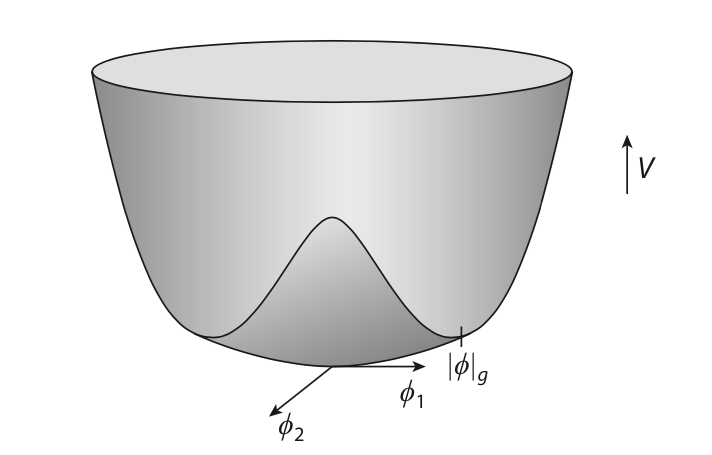
\includegraphics[width = 0.5\textwidth]{images/higgs-potential.png}
    \caption{Higgs potential from equation \eqref{eq:singlet_higgs_pot} in the complex plane (retrieved from \cite{goldberg_standard_2017}).}
    \label{fig:higgs}
\end{figure}

However, this  VEV is not unique, it is determined up to multiplication by a phase factor. This means that the Lagrangian for this scalar obeys a $U(1)$ symmetry. $SU(2)_L$ symmetry is further imposed by turning the scalar field into a doublet of the form $$\Phi = \mqty(\phi_1 \\ \phi_2),$$ called the Higgs doublet. To account for this new doublet structure, the Lagrangian from equation \eqref{eq:singlet_higgs_lag} becomes
\begin{equation}
    \mathcal{L} = \frac{1}{2}\dcov \Phi \dcon \Phi^\dagger - V(\Phi),
\end{equation}
with
\begin{equation}\label{eq:higgs_pot}
    V(\phi) = -\mu^2 \Phi\Phi^\dagger + \lambda(\Phi\Phi^\dagger)^2.
\end{equation}

As a gauge choice, let the VEV for the scalar doublet be
\begin{equation}
    \Phi_0 = \mqty (0 \\ \frac{v}{\sqrt{2}}),
\end{equation}
where $v=\mu/\sqrt{\lambda}$. The choice of the ground state spontaneously breaks the $U(1)$ symmetry of the potential, which entails the existence of two Goldstone bosons, one for each component of the doublet \cite{goldberg_standard_2017}. These Goldstone bosons can be seen when considering a small excitation of the Higgs doublet:
\begin{equation}
    \Phi =\mqty (\phi_1(x) \\ \frac{v+H(x)}{\sqrt{2}}e^{i\alpha(x)}),
\end{equation}
where $H$ and $\alpha$ are real scalar fields.
The scalar Lagrangian then expands to
\begin{equation}
    \lag = \dcov \phi_1 \dcon \phi_1^* + \frac{1}{2}\qty(v+H)^2 \dcov \alpha \dcon \alpha + \frac{1}{2}\dcov H \dcon H - \mu^2 H^2 + \text{self-interaction terms}.
\end{equation}
The $\phi_1$ Goldstone boson only interacts with itself and may be disregarded, while the $\alpha$ Goldstone boson interacts with itself and the $H$ boson. These terms are not of interest. The last two terms are however important: they represent a real scalar particle with mass $\mu = M_H$.

Returning to the $SU(2)_L\times U(1)$ symmetry, the weak hypercharge of the scalar doublet is taken as $Y_H = 1$ \cite{goldberg_standard_2017}, so it transforms under $SU(2)_L\times U(1)$ as
\begin{equation}
    \Phi \rightarrow e^{-ig'\theta^0/2}e^{-ig_W\theta_i\sigma_i/2}\Phi.
\end{equation}
As is the case for fermions, a local $SU(2)\times U(1)$ brings about interactions with gauge bosons via the covariant derivative 
\begin{equation}
    D_\mu = \dcov + i\frac{g'}{2}B_\mu + i \frac{g_W}{2} \sigma_i W^{i}_{\mu}.
\end{equation}
The Lagrangian for the scalar field becomes
\begin{equation}
    \lag_{\Phi} = D_\mu \Phi D^\mu \Phi^\dagger - V(\Phi).
\end{equation}
Ignoring the presence of Goldstone bosons, all off-diagonal terms in the kinetic part of the Lagrangian are zero. Thus, the covariant derivative introduces terms of the form
\begin{equation}
    \frac{1}{8}(v+H)^2\qty[\qty(g' B_\mu - g_W W_{\mu}^3)^2 + g_W^2(W^1)^2 + g_W^2(W^2)^2].
\end{equation}
Weinberg's rotation turns this expression into
\begin{equation}
    \lag_{\text{mass}} = \frac{1}{2} M_Z^2 Z_{\mu}Z^{\mu} + \frac{1}{2} M_W^2 W^+_{\mu} W^{-\;\mu},
\end{equation}
where
\begin{align}
    M_W &= \frac{M_H}{\sqrt{8\lambda}},\\
    M_Z &= \frac{M_W}{\cos{\theta_W}}.
\end{align}
This explains the mass of gauge bosons via the Higgs mechanism.

Fermion mass is obtained by introducing Yukawa interaction terms in the Lagrangian of the form
\begin{equation}
    -\lambda \overline{\psi} \Phi \psi.
\end{equation}
Upon splitting fermionic spinors into left- and right-handed components, allowing only terms that are gauge invariant, and relaxing the scalar doublet into the chosen ground state, these terms become
\begin{equation}
    -\lambda\frac{v}{\sqrt{2}}\overline{\psi}_L\overline{\psi}_R,
\end{equation}
which represent mass terms for the fermionic fields.

\subsubsection*{Strong interaction}


The symmetry group for the strong interaction is $SU(3)_C$, where $C$ stands for the coloured charge. Hence, the strong interaction is referred to as chromodynamics. Quarks come in three colours: red, blue and green. Thus, they are expressed as column vectors:
$$\psi = \mqty( q_r \\ q_b \\ q_g).$$
The free quark Lagrangian is
\begin{equation}
    \mathcal{L} = i \overline{\psi}_i\gamma^\mu \dcov \psi_i-m_i\overline{\psi}_i\psi_i,
\end{equation}
where the index stands for the flavour of the quark. There are six quark flavours: up, down, strange, charm, top, and bottom.

We now incorporate the symmetry in the Lagrangian. A general $SU(3)$ transformation is of the form
\begin{equation}
    \psi \rightarrow e^{-ig_s\theta_a\lambda_a} \psi,
\end{equation}
where $\lambda_a$ are the eight generators of the $SU(3)$ Lie algebra. The corresponding Noether current is
\begin{equation}
    J^{(a)\mu} = g_s \overline{\psi}\gamma^\mu\lambda_a \psi.
\end{equation}
As in $SU(2)$, the gauge invariant fields are transform by
\begin{equation}
    G_{\mu}^{a} \rightarrow G_{\mu}^{a} + \dcov \theta^a - 2 \sum_{j,k} f^{a jk}G_{\mu}^{j}\theta^{k},
\end{equation}
where $f^{ijk}$ are the structure constants of the $SU(3)$ Lie algebra. These fields are known as gluon fields. The covariant derivative is 
\begin{equation}
    D_\mu = \dcov +\frac{i}{2}g_s\lambda_{a}G_{\mu}^{a}.
\end{equation}
The Faraday tensor for gluons is
\begin{equation}
    F_{\mu\nu}^{a} = D_\mu G_\nu^a - D_\nu G_\mu ^a = \dcov G_\nu^a -\dcov[\nu] G_{\mu}^a +2g_s\sum_{jk}f^{jkl}G_{\mu}^{k}G_\nu^{l}.
\end{equation}
This results in the chromodynamic Lagrangian:
\begin{equation}
    \mathcal{L}_\text{S} = \overline{\psi}(i\gamma^\mu\dcov-m)\psi-G_\mu^{a}J^{(a)\mu}-\frac{1}{16}F^{(k)\mu\nu}F_{(k)\mu\nu}.
\end{equation}

\section{Beyond the SM: Leptoquark physics}

As claimed in chapter \ref{ch:chapter1}, the main motivation for introducing leptoquarks is that they provide an explanation for LFU violation, as hinted by experimental $B$-meson decay anomalies \cite{lhcb_measurement,lhcbcollaboration2021test}. Although there is a plethora of combined explanations for these anomalies in the literature (see for instance \cite{buttazzo_b-physics_2017, calibbi_effective_2015, bhattacharya_simultaneous_2015, alonso_lepton_2015}), mainly within the Effective Field Theory (EFT) framework, many of them exhibit serious issues such as a breakdown of the perturbative expansion, missing ultra-violet (UV) completion, and excess tuning of parameters \cite{di_luzio_maximal_2018}. Moreover, few models are consistent with high transverse momentum ($p_T$) constraints, as outlined in \cite{faroughy_confronting_2017, greljo_high-p_tdilepton_2017}, and other experimental (non-)observations \cite{di_luzio_gauge_2017}. Nonetheless, the literature has singled out a vector leptoquark in the $(3,1,2/3)$ representation of the SM gauge group coupled mainly to third-generation fermions as a simple addition to the SM which explains all anomalies and is consistent with low-energy data \cite{buttazzo_b-physics_2017}. A crucial feature of this representation is the absence of down-quark-to-neutrino or up-quark-to-charged-lepton transitions \cite{di_luzio_gauge_2017}. In other explanations for the anomalies, suppression of these interactions requires stringent and often unnatural constraints on the model. However, the inclusion of a massive vector field requires a UV completion. This section reviews a subset of the literature devoted to embedding the $(3,1,2/3)$ leptoquark in suitable UV completion.

There are two ways a UV-complete theory may produce massive vectors: composite dynamics \cite{barbieri_anomalies_2016} or a spontaneously broken gauge symmetry. The former approach although plausible and theoretically consistent with precision electroweak measurements, it exhibits renormalisation issues \cite{di_luzio_gauge_2017}. Hence, the latter approach is followed. Consider the gauge group $G = SU(4)\times SU(3)' \times SU(2)_L \times U(1)'$. The model arising from this gauge structure is known as the 4321 model, due to the degree in each factor, and is constructed following a bottom-up approach. The experimental anomalies require the following effective interaction terms with SM fermions:
\begin{equation}\label{eq:LQ-fermion-lag}
    \mathcal{L} \supset \frac{g_U}{\sqrt{2}} U_{1}^{\mu,\alpha} \qty[\beta_{L}^{ij}\overline{q}_L^{i,\alpha}\gamma_\mu \ell^{j}_{L} + \beta_{R}^{ij}\overline{d}_R^{i,\alpha}\gamma_\mu e^{j}_{R}] + \mathrm{h.c.},
\end{equation}
where $U_1^\mu$ is the vector leptoquark, $q_L (\ell_L)$ denotes left-handed quark (lepton) doublets, $d_R (e_R)$ denotes right-handed down-type quark (charged-lepton) singlets, $i,j\in\{1,2,3\}$ are family indexes, $\alpha\in \{1,2,3\}$ are $SU(3)_c$ colour indices and $\beta^{ij}_{L/R}$ are complex matrices. These terms in turn fix the SM representation for the $U_1$ vector as $(3,1,2/3)$. The minimal group $G_{\mathrm{min}} \supset G_{\mathrm{SM}}$ that contains generators transforming under this representation is \cite{baker_high_2019}, 
\begin{equation}\label{eq:G-min1}
    G_{\mathrm{min}} = SU(4) \times SU(2)_L \times U(1)_{T_R^3}.
\end{equation}
$G_{\mathrm{min}}$ is obtained as a subgroup of the Pati-Salam group \cite{pati_lepton_1974}, $$ G_{\mathrm{PS}} = SU(4) \times SU(2)_L \times SU(2)_R,$$ by defining $U(1)$ to be the subgroup of $SU(2)_R$ defined by the diagonal (electric-charge neutral) generator $T_R^3$. However, the minimal group from \eqref{eq:G-min1} constraint the coupling constants so much that there is no freedom to comply with low-energy and high-energy data \cite{baker_high_2019}. This is issue is averted by the next-to-minimal gauge group, $$G = SU(4)\times SU(3)' \times SU(2)_L \times U(1)_{T_R^3}.$$


% On the other hand, there is a purely theoretical perspective presented in \cite{di_luzio_gauge_2017}. The chiral structure of the SM suggests the Pati-Salam (PS) model with gauge structure $$G_{\text{PS}} = SU(4)_{\text{PS}} \times SU(2)_L \times SU(2)_R.$$ However, this model puts the LQ mass close to $100\;\si{TeV}$, meaning it could not explain low-energy LFU violations.

\subsection{Features of the 4321 Model}

It is clear that the 4321 extends the SM group by an extra $SU(4)$ factor. However, the embedding of $G_{\text{SM}}$ in the 4321 group is not that straightforward: the $SU(3)_c$ factor is identified with a diagonal subgroup, namely $$\qty(SU(3)_4 \times SU(3)')_{\mathrm{diag}},$$ where $SU(3)_4\times U(1)_4 \subset SU(4)$. Similarly, $$U(1)_Y = (U(1)_4\times U(1)')_{\mathrm{diag}}.$$ This embedding produces certain relationships between the $G_{\mathrm{SM}}$ generators and those of the larger group. Let $T_{\alpha}$ ($\alpha = 1,\dotsc,15$) denote the fifteen generators\footnote{The Lie algebra of $SU(N)$ has $N^2-1$ generators \cite{hall_lie_2015}} of $SU(4)$, then $$Y = \sqrt{\frac{2}{3}} T_{15} + Y',$$ where $T^{15} =  (2\sqrt{6})^{-1} \mathrm{diag}(1,1,1,-3)$.

Naturally, the larger gauge group should bring about new interactions with new mediators. These arise as generators of the quotient group $G_{4321}/G_{\mathrm{SM}}$ and transform under $G_{\mathrm{SM}}$ as $U_1\sim (3,1,2/3)$, $g'\sim (8,1,0)$ and $Z'\sim (1,1,0)$ \cite{di_luzio_maximal_2018, di_luzio_gauge_2017}. Notice that the $U_1$ has the desired transformation properties of the vector leptoquark, while the $g'$ and $Z'$ gauge fields transform just like the SM gluon and $Z$ boson. The spontaneous breaking of $G_{4321}$ into $G_{\mathrm{SM}}$ gives these vectors their mass via the Higgs mechanism. Moreover, the $U_1$ and $Z'$ vectors interact in a flavour-non-universal fashion with fermions. Such interactions can be produced in two ways: by introducing Cabbibo mixing between SM fermions and exotic fermions, as proposed in \cite{di_luzio_gauge_2017}, or by having flavour-dependent $SU(4)\times SU(3)'$ quantum numbers \cite{bordone_three-site_2018, greljo_third_2018}. In either case, the $B$-meson anomalies can be fully explained and allow for a leptoquark mass within a few TeV. 

To conclude this section, the Lagrangian in this model produces the following terms related to the vector leptoquark:
\begin{equation}\label{eq:U1-lag}
    \begin{aligned}
        \mathcal{L}_{U_{1}}=&-\frac{1}{2} U_{1 \mu \nu}^{\dagger} U_{1}^{\mu \nu}+M_{U}^{2} U_{1 \mu}^{\dagger} U_{1}^{\mu} \\
        &-i g_{s}\left(1-\kappa_{U}\right) U_{1 \mu}^{\dagger} T^{a} U_{1 v} G^{a \mu v} \\
        &-i g_{Y} \frac{2}{3}\left(1-\tilde{\kappa}_{U}\right) U_{1 \mu}^{\dagger} U_{1 v} B^{\mu v} \\
        &+\frac{g_{U}}{\sqrt{2}}\left[U_{1}^{\mu}\left(\beta_{L}^{i j} \bar{q}_{L}^{i} \gamma_{\mu} \ell_{L}^{j}+\beta_{R}^{i j} \bar{d}_{R}^{i} \gamma_{\mu} e_{R}^{j}\right)+\text { h.c. }\right]
    \end{aligned}
\end{equation}

The first line of \eqref{eq:U1-lag} includes the free, massive vector boson terms. The second and third lines represents leptoquark coupling with the colour sector, $SU(3)_C$, and with the $U(1)_Y$ gauge boson, respectively. The last line includes terms responsible for vertices like that shown in figure \ref{fig:vertex}. These are exactly the terms from \eqref{eq:LQ-fermion-lag} that are necessary for explaining the $B$-meson anomalies using a vector leptoquark \cite{baker_high_2019}.

\begin{figure}
    \centering
    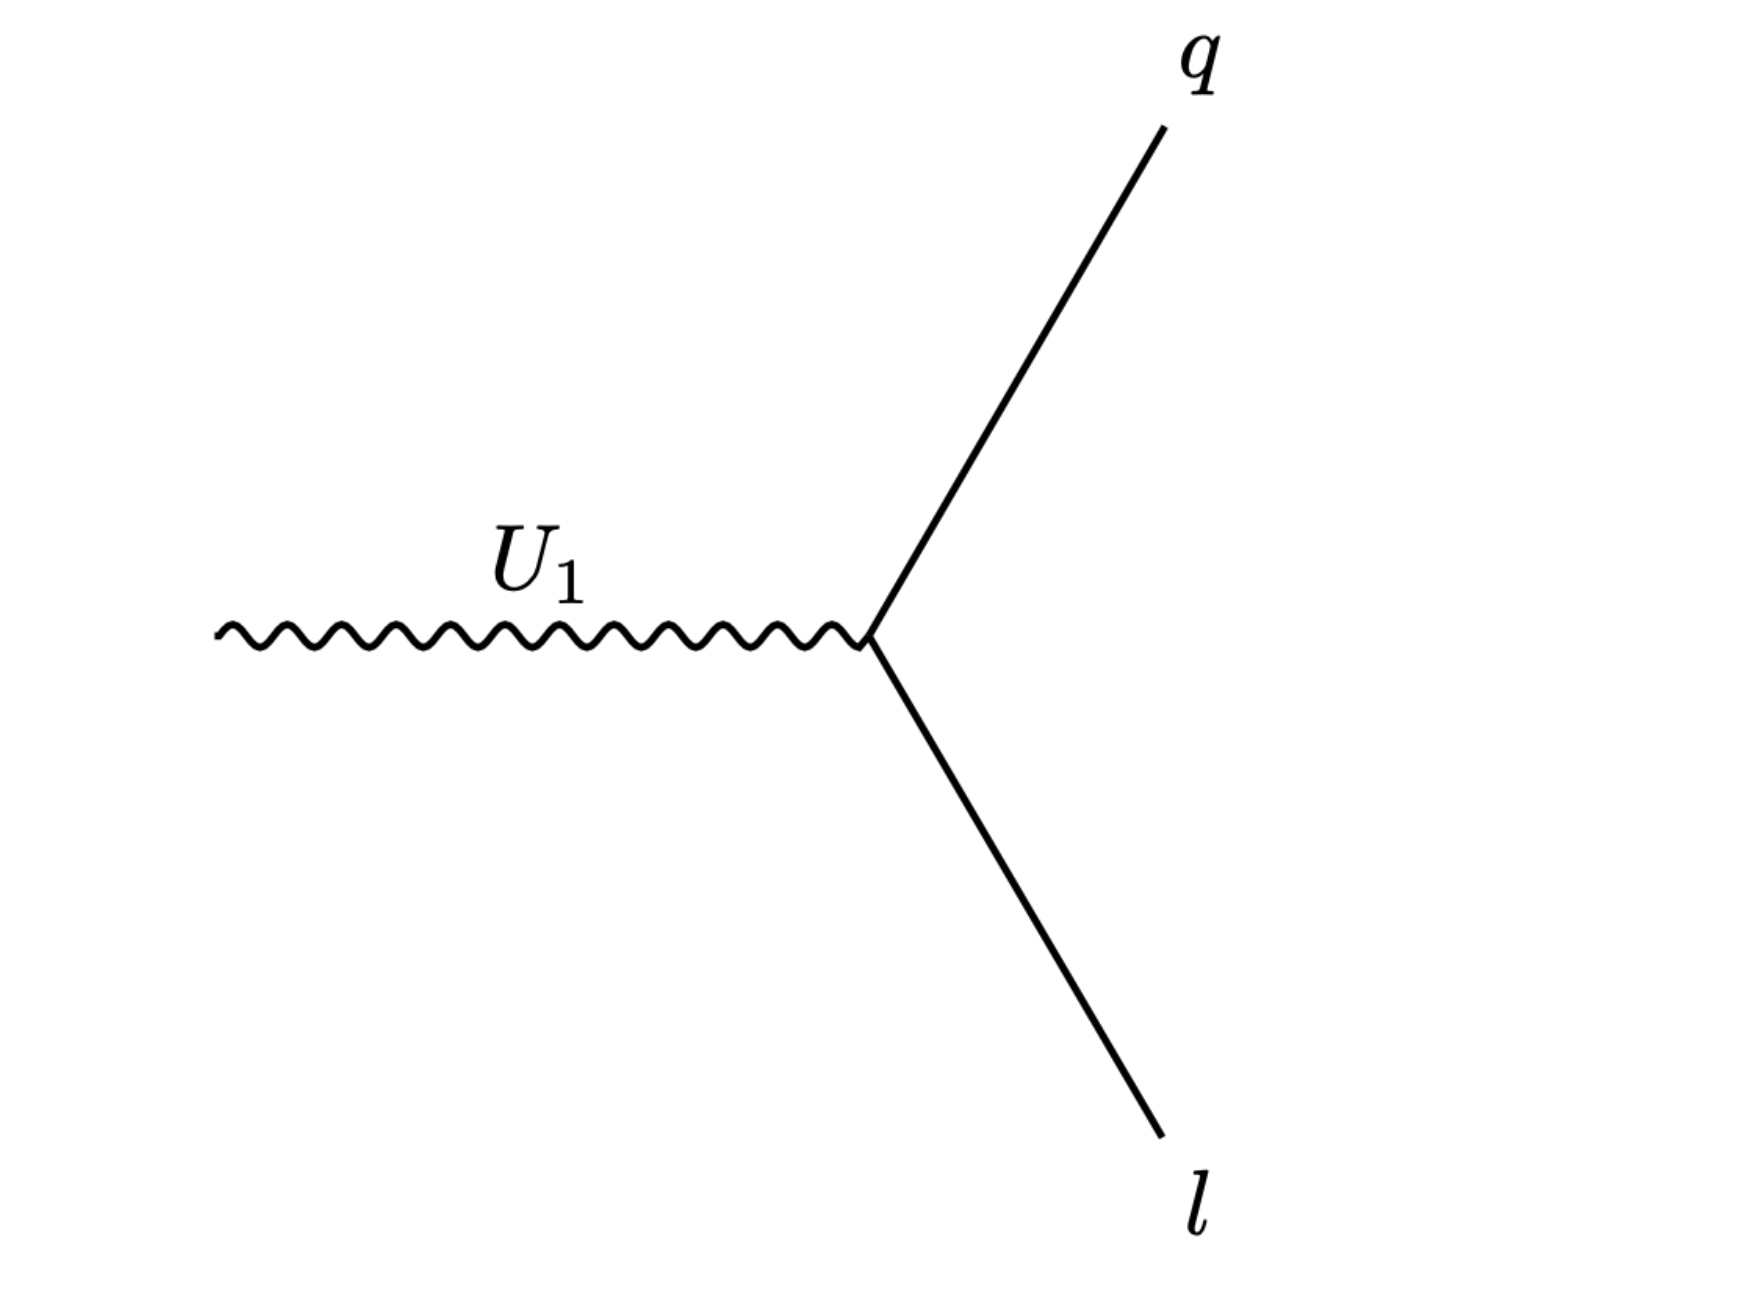
\includegraphics[width = 0.5\textwidth]{images/lq-vertex.png}
    \caption{Feynman diagram vertex showing a vector leptoquark ($U_1$) coupling to a quark $q$ and a lepton $l$.}
    \label{fig:vertex}
\end{figure}



